\documentclass[11pt, a4paper]{article}

\usepackage{biblatex}
\usepackage{classicthesis}
\usepackage{graphicx}
\usepackage[margin=1in]{geometry}
\usepackage{pdflscape}
\usepackage{sectsty}
\usepackage{tocloft}


% Bibliography and table of contents
\addbibresource{biblio.bib}

% Customize sections
\allsectionsfont{\Large}
\renewcommand{\cftsecfont}{\bfseries} % Apply bold to sections
\renewcommand{\cftsecpagefont}{\bfseries} % Apply bold to number pages
\renewcommand{\cftsecleader}{\cftdotfill{\cftdotsep}} % Separate with dots


% Title and author
\title{\normalfont\spacedallcaps{Database design for transportation company}}

\author{\spacedlowsmallcaps{CarlosFOL}} 

\date{}


% Body
\begin{document}

\pagenumbering{gobble}

\maketitle



\tableofcontents

\vspace{2in}

\begin{figure}[h!]
    \centering
    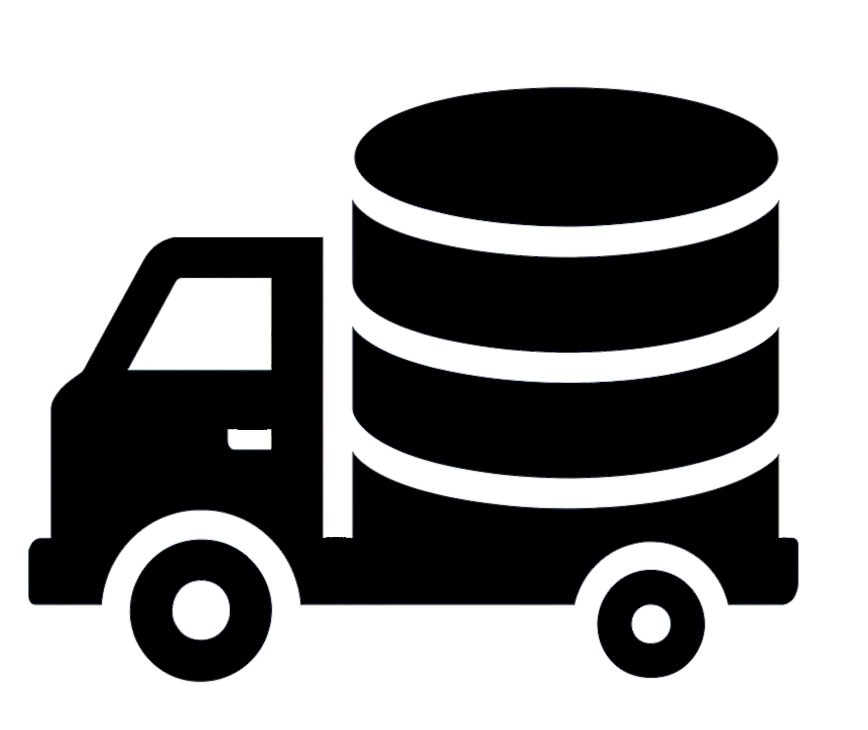
\includegraphics[width=0.5\textwidth]{img/logo.png}
    \label{logo_db}
\end{figure}


\newpage

\pagenumbering{arabic}

\section{Description of the problem}

The transportation company needs a comprehensive database system to record and manage daily trips with an exhaustive level of detail. This system must provide an integral tool that allows detailed, precise, and comprehensive tracking of every operational and financial aspect of the transport company's trips.\\

\subsection{Trip Information}
Each trip is characterized by a unique code that distinguishes it from others, allowing for precise tracking of operations. The system captures the complete temporality of the trip, recording both the start and end dates, which provides a clear temporal framework for each movement.\\

Each trip is associated with a specific purpose, which includes name, description, and a unique code. For example, a type of purpose could be "goods transportation," while a specific purpose would be "transportation of vehicle chassis to branch B." The current status of the trip is recorded in detail, allowing real-time tracking of operations.\\

It is essential for the system to maintain complete traceability of vehicles, drivers, and their association with trips. The system must track which driver operates each vehicle within that trip, recording arrival dates, departure dates, and whether there were delays in the start.\\

Another critical element is the remittance guide, provided by the customer. A unique code for this document is registered, which the driver must have as proof of delivery. This mechanism ensures the traceability and accountability of each trip.\\

\subsection{Geographic Information}
Geographic location plays a fundamental role in the registration. Each point in the system is saved with a unique code, precise coordinates (latitude and longitude), a descriptive name, and a complete address (including street, number, council, postal code, and country). The system precisely documents both the origin and destination points of each route.\\

Each defined route (origin-destination pair) is assigned a unique route identifier in the system, making it possible to reference and track specific routes precisely. Each of these routes has a specific tariff established in the system and can be classified as local if both its origin and destination belong to the same province. Otherwise, it is considered regional.\\

The company's pricing model is based on predefined route tariffs. Any other factor that might impact the final service cost is considered an additional expense, categorized by type.\\

\subsection{Vehicle Information}
Regarding vehicles, the system manages comprehensive information. Each unit is identified by a unique chassis number. Complete characteristics are registered such as brand, model, color, and vehicle family. The vehicle's condition is documented, differentiating between new and used units, which allows for more efficient fleet management.\\

The system maintains a comprehensive tracking history of each vehicle's Technical Inspection documentation. This includes registering the inspection code, issue date, and expiration date of the certificate, as well as tracking whether the inspection is current. This historical tracking is crucial for maintaining safety and regulatory compliance of the transport fleet.\\

A vehicle can be owned either by the transportation company itself or by a customer. It's important to note that not all vehicles belong to customers—many belong to the transportation company itself.\\

\subsection{Driver Information}
Driver management is another fundamental aspect of the system. Each driver is identified by a unique ID and has attributes including their full name. The system tracks each driver's license details, including the license ID, issue date, expiration date, and type. The system also monitors whether the license is current.\\

\subsection{Customer Information}
Customer management is carried out with an equally detailed level. Each customer is registered with a unique identifier (TIN) and corresponding name. The system allows customers to schedule trips, providing complete operational flexibility.\\

\newpage

\newgeometry{left=0.5in, bottom=0.2in}

\begin{landscape}

\section{Entity-Relationship model}

\begin{figure}[h!]
    \centering
    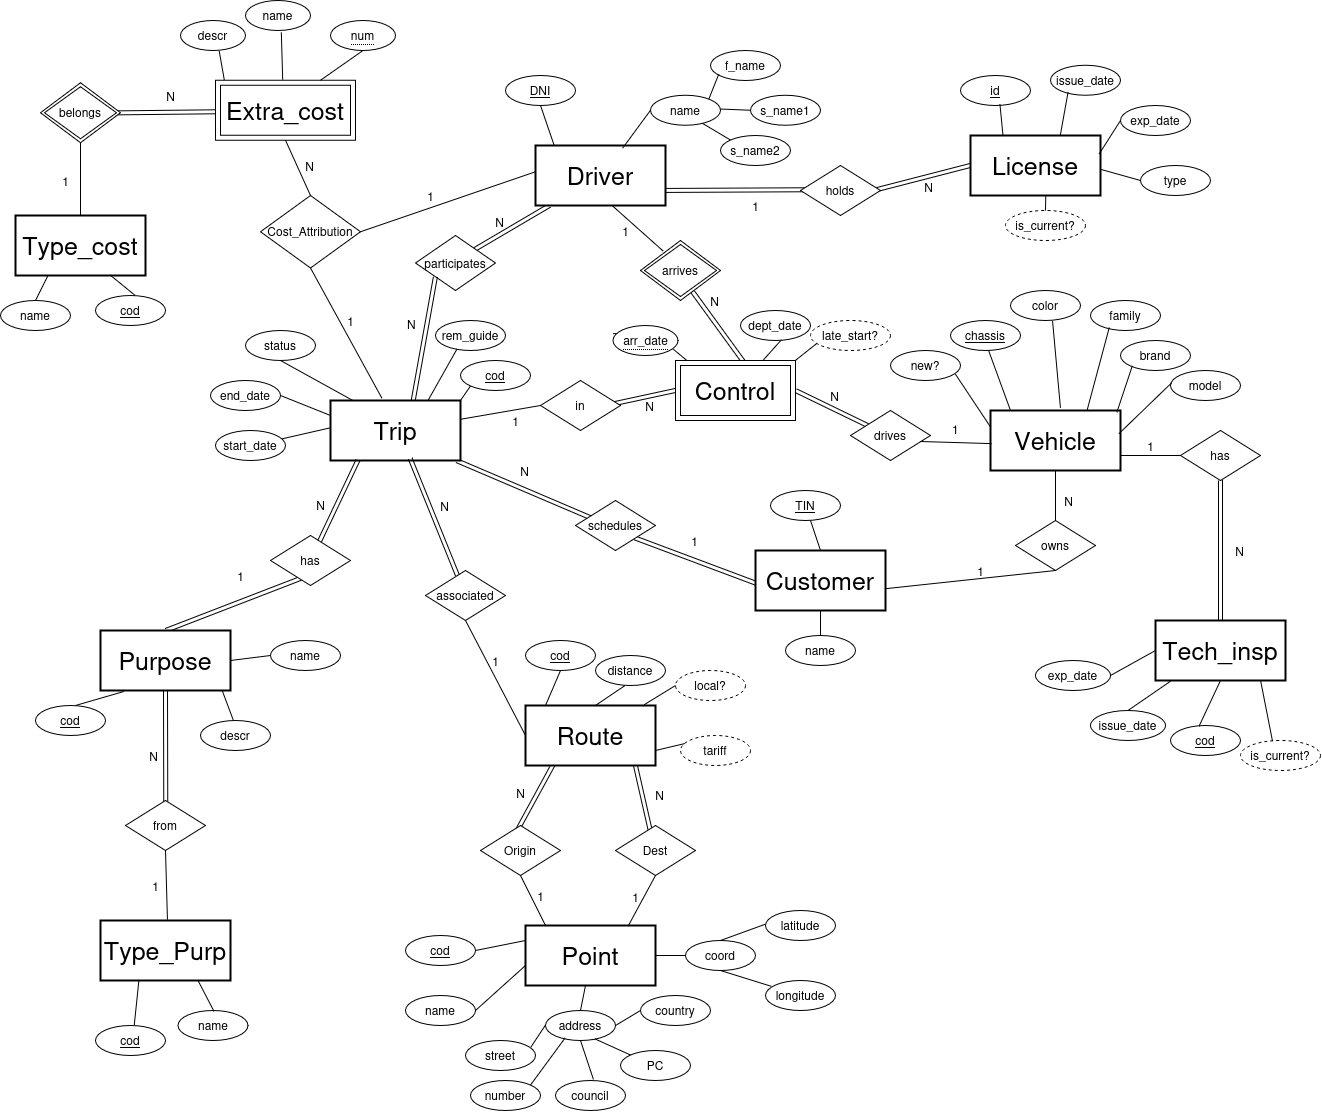
\includegraphics[width=1.03\textwidth]{img/er_model.png}
    \caption{ER model}
    \label{er_model}
\end{figure}
    

\end{landscape}


\newpage

\restoregeometry

\section{Logical schema}

The graphical interface of \href{https://www.supabase.com}{Supabase} was used to generate the following diagram:


\end{document}
